%%%%%%%%%%%%%%%%%%%%%%%%%%%%%%%%%%%%%%%%%
% a0poster Landscape Poster
% LaTeX Template
% Version 1.0 (22/06/13)
%
% The a0poster class was created by:
% Gerlinde Kettl and Matthias Weiser (tex@kettl.de)
% 
% This template has been downloaded from:
% http://www.LaTeXTemplates.com
%
% License:
% CC BY-NC-SA 3.0 (http://creativecommons.org/licenses/by-nc-sa/3.0/)
%
%%%%%%%%%%%%%%%%%%%%%%%%%%%%%%%%%%%%%%%%%

%----------------------------------------------------------------------------------------
%	PACKAGES AND OTHER DOCUMENT CONFIGURATIONS
%----------------------------------------------------------------------------------------

\documentclass[a0,landscape]{a0poster}


\usepackage{multicol} % This is so we can have multiple columns of text side-by-side
\columnsep=80pt % This is the amount of white space between the columns in the poster
\columnseprule=3pt % This is the thickness of the black line between the columns in the poster

\usepackage[svgnames]{xcolor} % Specify colors by their 'svgnames', for a full list of all colors available see here: http://www.latextemplates.com/svgnames-colors

\usepackage{times} % Use the times font
%\usepackage{palatino} % Uncomment to use the Palatino font

\usepackage{graphicx} % Required for including images
\graphicspath{{figures/}} % Location of the graphics files
\usepackage{booktabs} % Top and bottom rules for table
\usepackage[font=small,labelfont=bf]{caption} % Required for specifying captions to tables and figures
\usepackage{amsfonts, amsmath, amsthm, amssymb} % For math fonts, symbols and environments
\usepackage{wrapfig} % Allows wrapping text around tables and figures

\usepackage{xcolor}

\usepackage{mdframed}      % breakable framed boxes with background
\usepackage{etoolbox}      % \AtBeginEnvironment / \AtEndEnvironment
\usepackage{multicol}      % example showing column wrapping (optional)

% Your theorem/definition setup (unchanged)
\newtheorem{theorem}{Theorem}
\theoremstyle{definition}
\newtheorem{definition}{Definition}

% Define colors
\definecolor{lightgreen}{RGB}{220,255,220}
\definecolor{lightgray}{RGB}{245,245,245}

% mdframed settings for the body only (no visible frame, only background)
\newmdenv[
  backgroundcolor=lightgray,
  linecolor=lightgray,    % same as background -> no visible border
  innerleftmargin=16pt,
  innerrightmargin=16pt,
  innertopmargin=14pt,
  innerbottommargin=14pt,
  skipabove=\topsep,
  skipbelow=\topsep,
  nobreak=false,
  splittopskip=14pt,
  splitbottomskip=14pt
]{defbodybox}

\newmdenv[
  backgroundcolor=lightgreen,
  linecolor=lightgreen,
  innerleftmargin=16pt,
  innerrightmargin=16pt,
  innertopmargin=14pt,
  innerbottommargin=14pt,
  skipabove=\topsep,
  skipbelow=\topsep,
  nobreak=false,
  splittopskip=14pt,
  splitbottomskip=14pt
]{thmbodybox}

% in preamble
\setlength{\abovedisplayskip}{12pt}
\setlength{\belowdisplayskip}{12pt}
\setlength{\abovedisplayshortskip}{12pt}
\setlength{\belowdisplayshortskip}{12pt}


% Surround only the *body* of the existing environments.
% The theorem/definition header produced by \begin{definition} stays outside the colored box.
\AtBeginEnvironment{definition}{\begin{defbodybox}\ignorespaces}
\AtEndEnvironment{definition}{\end{defbodybox}}

\AtBeginEnvironment{theorem}{\begin{thmbodybox}\ignorespaces}
\AtEndEnvironment{theorem}{\end{thmbodybox}}

\usepackage{tikz}
\usetikzlibrary{positioning,shapes.geometric}

\DeclareMathOperator*{\argmax}{arg\,max}

\begin{document}

%----------------------------------------------------------------------------------------
%	POSTER HEADER 
%----------------------------------------------------------------------------------------

% The header is divided into three boxes:
% The first is 55% wide and houses the title, subtitle, names and university/organization
% The second is 25% wide and houses contact information
% The third is 19% wide and houses a logo for your university/organization or a photo of you
% The widths of these boxes can be easily edited to accommodate your content as you see fit



\begin{minipage}[b]{\linewidth}
\Huge \color{NavyBlue} \textbf{Improving Robustness to Model Misspecification in Bayesian Experimental Design} \color{Black}\\ % Title
\huge\textit{Alexander J. Forster, Desi R. Ivanova, Tom Rainforth}\\[0.5cm] % Subtitle
\large \textbf{Jhonathan Navott, Tobias Bretschneider, Jakob Hartmann}\\ % Author(s)
%\huge Fundamentals of AI (EIT CDT)\\ % University/organization
\end{minipage}


\vspace{-1cm} % A bit of extra whitespace between the header and poster content

%----------------------------------------------------------------------------------------

\begin{multicols}{4} % This is how many columns your poster will be broken into, a poster with many figures may benefit from less columns whereas a text-heavy poster benefits from more

%----------------------------------------------------------------------------------------
%	ABSTRACT
%----------------------------------------------------------------------------------------

\color{Navy} % Navy color for the abstract

\begin{abstract}

We discuss the approach of Forster et al. (2025)~\cite{forster_improving_2025}, in improving robustness to model misspecification in Bayesian experimental design. Their approach builds the misspecification into the optimal design paradigm. We discuss their main results, replicate their experiments, and extend upon them by examining how the flexibility of the auxiliary model effects the robustness of this method.
%%% Needs more detail! - ADDED some, but I don't think the last part I wrote is is brilliantly written
\end{abstract}
\color{SaddleBrown} % SaddleBrown color for the introduction

\section*{Motivation}

Bayesian experimental design (BED) is a commonly used method to efficiently select new data samples to maximise information gain about the model parameters \cite{smith_prediction-oriented_2023}. However, if the model is misspecified (i.e. cannot fit the true data generating process) then BED can fail spectacularly. For real world applications it is often the case that the model is misspecified, and thus BED is not necessarily applicable.  One naive solution could be choosing a more flexible model class, however this discarded any useful prior information; making the problem harder to learn. The authors of \cite{forster_improving_2025}, suggest a more robust method by integrating the assumption of misspecification into the design process. To do this they build an extended model, mixing a flexible auxiliary model with the parametrised model. 


\color{DarkSlateGray} % DarkSlateGray color for the rest of the content

\section*{Preliminaries}

% We have four different models, each modelling an experiment output $y \in \mathcal{Y}$ given a specific experimental design $\xi \in \mathcal{X}$. These are:

% \begin{definition}[Assumed model]
% The assumed (possibly misspecified) parametric model is
% \[
% y \sim p_{\mathrm{model}}(y \mid \theta, \xi),
% \]
% where $\theta \sim p_\theta(\cdot)$ are the unknown model parameters.
% \end{definition}
% \begin{definition}[Auxiliary model]
% The auxiliary model,
% \[
% y \sim p_{\mathrm{aux}}(y \mid \varphi, \xi)
% \]
% governed by parameters $\varphi \sim p_\varphi(\cdot)$.
% \end{definition}
% \begin{definition}[Extended model]
% The mixture of the two,
% \[\begin{aligned}
% Z &\sim \mathrm{Bernoulli}(1-\varepsilon),\\[4pt]
% y &\sim
% \begin{cases}
% p_{\mathrm{model}}(\,y\mid \theta,\xi) & \text{if } Z=1,\\[4pt]
% p_{\mathrm{aux}}(\,y\mid \psi,\xi)   & \text{if } Z=0, \text{ and;}
% \end{cases}
% \end{aligned}
% \]
% \end{definition}
% \begin{definition}[True model]
% The true model, $p_{\text{true}}(\,y\mid \xi\,).$
% \end{definition}

\begin{definition}[The models]
We next define four models, each modelling an experiment output $y \in \mathcal{Y}$ given a specific experimental design $\xi \in \mathcal{X}$. These are:
\begin{itemize}
\item The assumed (possibly misspecified) parametric model is
\[
y \sim p_{\mathrm{model}}(y \mid \theta, \xi),
\]
where $\theta \sim p_\theta(\cdot)$ is our prior over the model parameters;
\item The auxiliary model,
\[
y \sim p_{\mathrm{aux}}(y \mid \varphi, \xi)
\]
governed by parameters $\varphi \sim p_\varphi(\cdot)$;
\item The mixture of the two, for $Z \sim \mathrm{Bernoulli}(1-\varepsilon)$
\[\begin{aligned}
% Z &\sim \mathrm{Bernoulli}(1-\varepsilon),\\[4pt]
y &\sim
\begin{cases}
p_{\mathrm{model}}(\,y\mid \theta,\xi) & \text{if } Z=1,\\[4pt]
p_{\mathrm{aux}}(\,y\mid \psi,\xi)   & \text{if } Z=0, \text{ and;}
\end{cases}
\end{aligned}
\]
\item The true model, $p_{\text{true}}(\,y\mid \xi\,).$
\end{itemize}
\end{definition}

With these in mind, we visualise the following possible configurations: The assumed model is well specified (case 1), the assumed model is misspecified and the auxiliary model is well specified (case 2), or the assumed model and auxiliary model are misspecified (case 3). The robust method developed in \cite{forster_improving_2025} is only valid for cases 1,2.

% \begin{minipage}[b]{0.6\linewidth}
\begin{center}
  \resizebox{13cm}{!}{%
    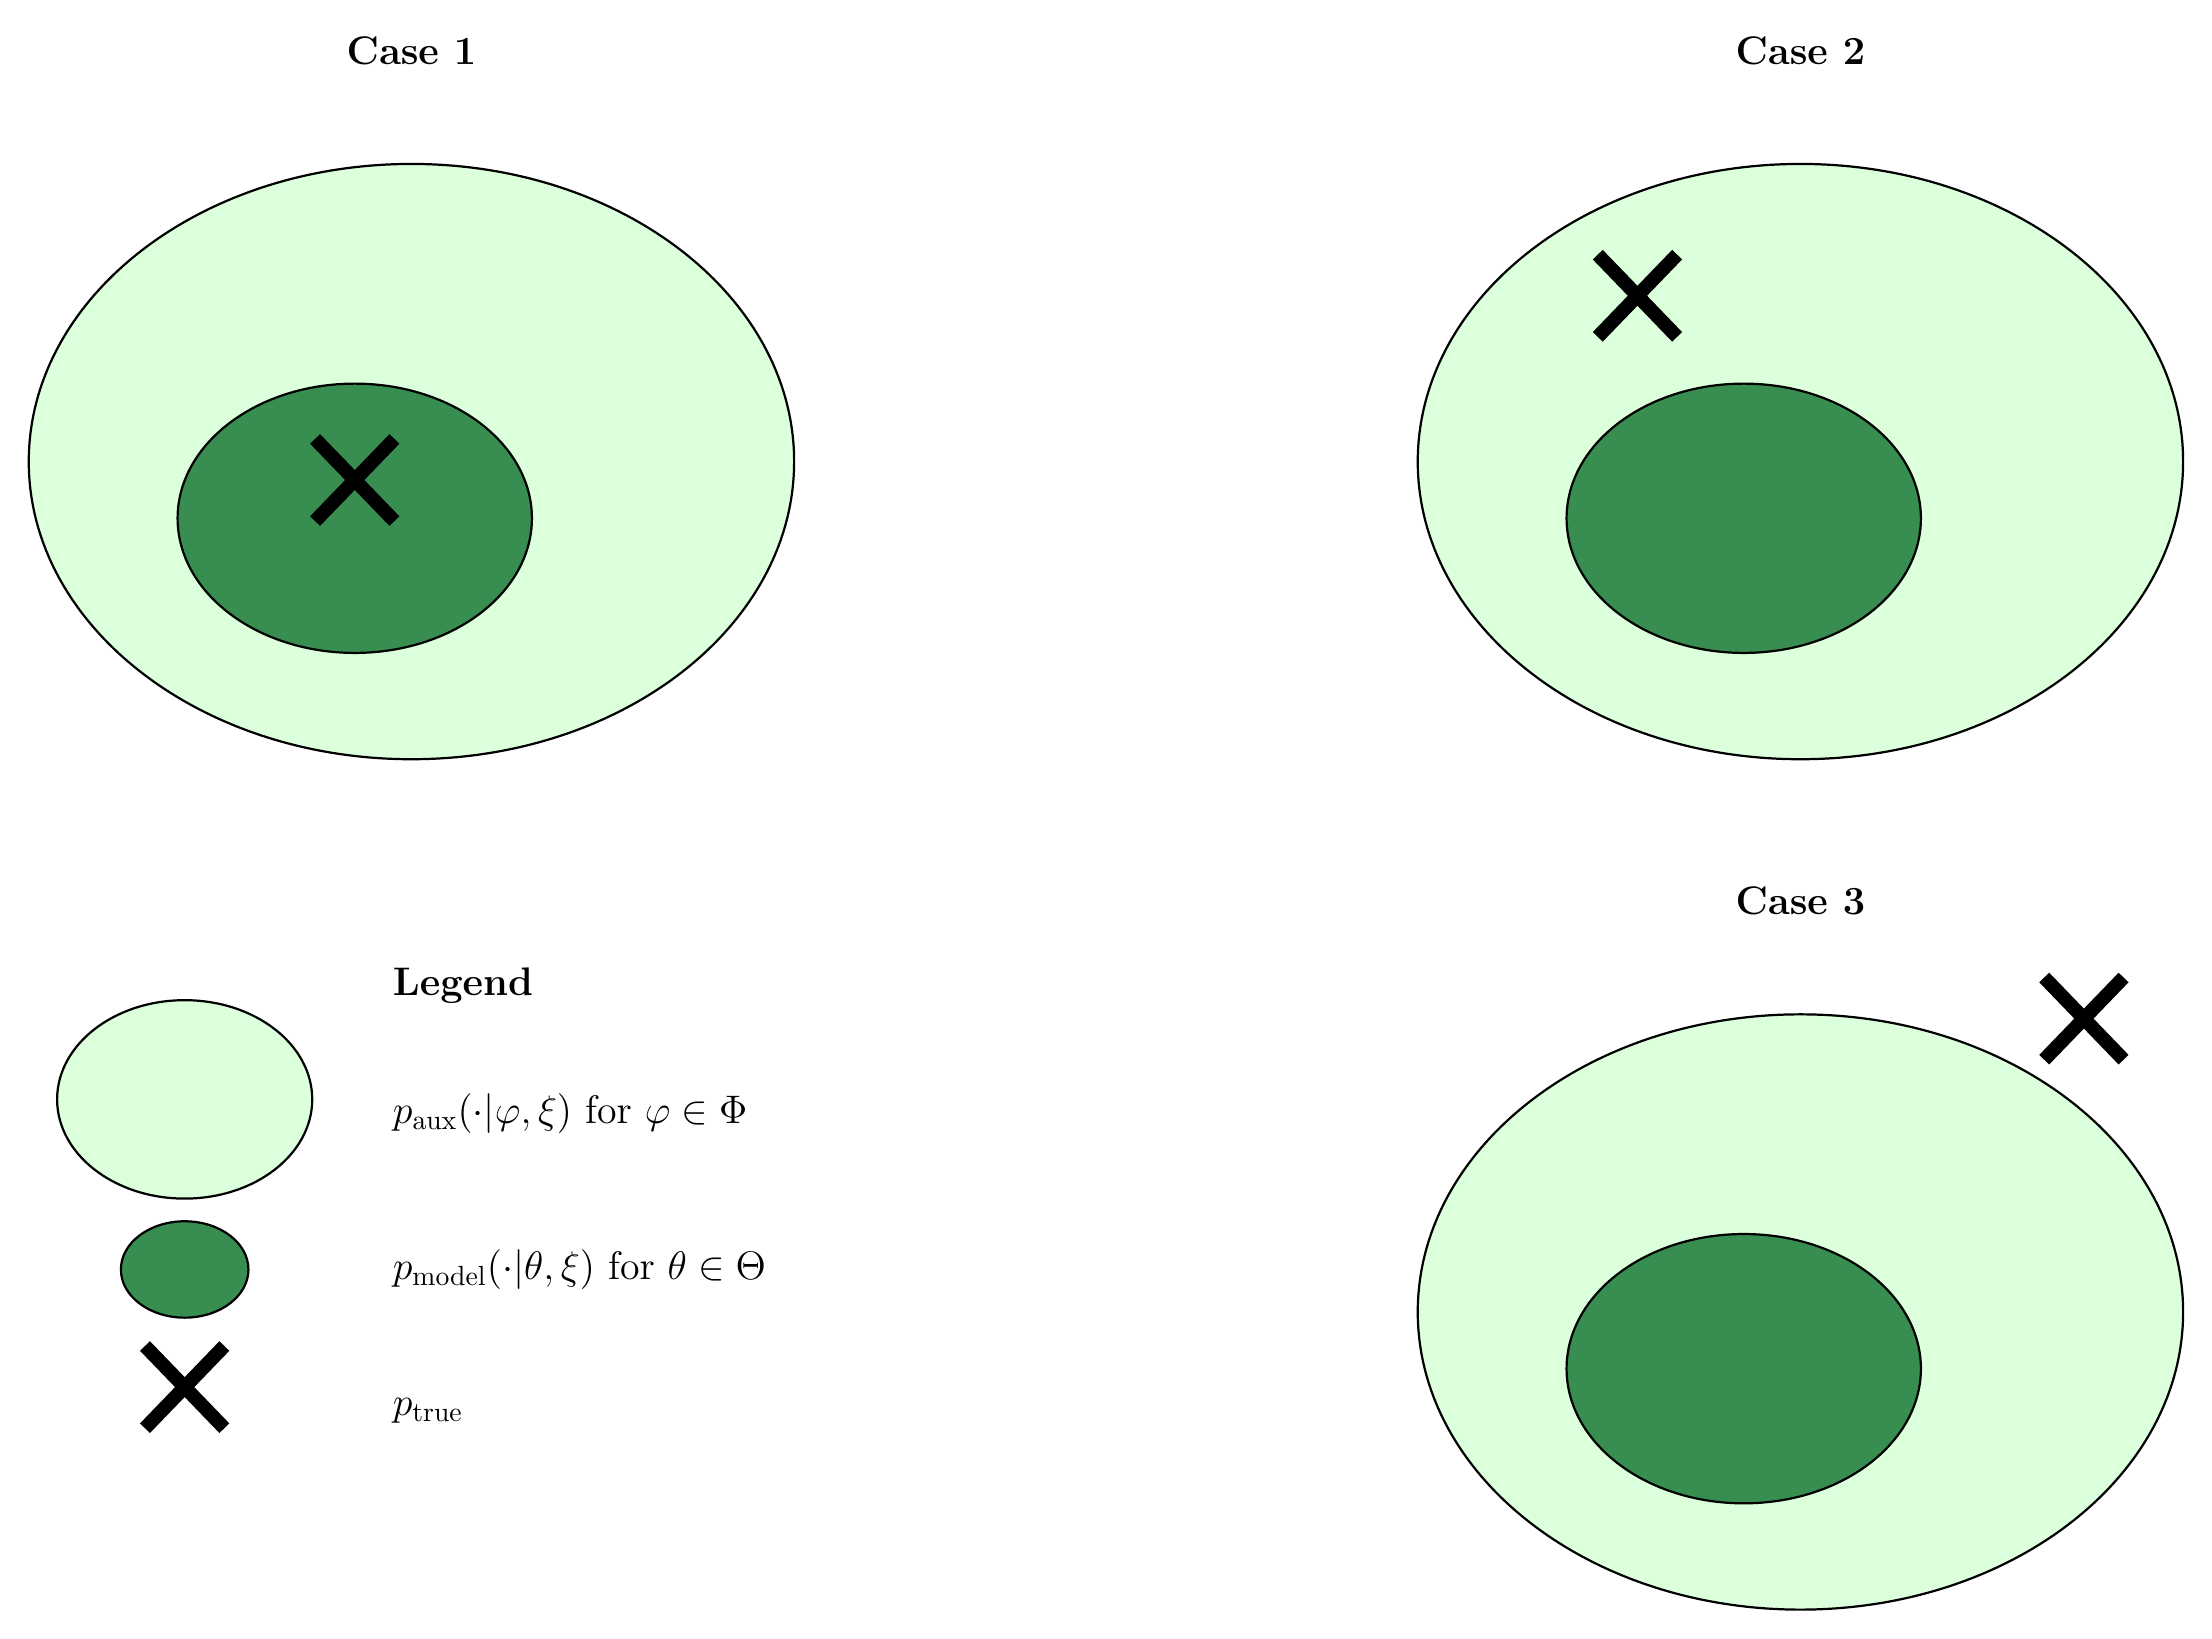
\begin{tikzpicture}[font=\sffamily, >=stealth]

      % Colors: light and dark green
      %\definecolor{auxfill}{RGB}{212,237,218}   % light green
      \definecolor{auxfill}{RGB}{220,255,220}

      \definecolor{modelfill}{RGB}{56,142,80}   % darker green

      % scale factor to make whole thing slightly bigger
      \def\myscale{1.8}

      % --- Top-left panel: Case 1 ---
      \begin{scope}[scale=\myscale, shift={(-5.0,3.2)}]
        % header
        \node[font=\bfseries\Large] at (0,2.9) {Case 1};

        % outer ellipse: p_aux (phi)
        \fill[auxfill] (0,0) ellipse (2.7cm and 2.1cm);
        \draw[thick] (0,0) ellipse (2.7cm and 2.1cm);

        % inner ellipse: p_model (theta)
        \fill[modelfill] (-0.4,-0.4) ellipse (1.25cm and 0.95cm);
        \draw[thick] (-0.4,-0.4) ellipse (1.25cm and 0.95cm);

        % % inner labels
        % \node[below=18pt, font=\Large] at (0,0) {$p_{\mathrm{model}}(\cdot;\theta)$};
        % \node[below=36pt, font=\Large] at (0,0) {$p_{\mathrm{aux}}(\cdot;\phi)$};

        % % p_true marker inside p_model (large X) and label
            \begin{scope}[shift={(-0.4,-0.4)}]
          \draw[line width=5pt] (-0.28,-0.02) -- (0.28,0.56);
          \draw[line width=5pt] (-0.28,0.56) -- (0.28,-0.02);
        \end{scope}
        % \node[right=6pt, font=\Large] at (0.75,0.25) {$p_{\mathrm{true}}$};
      \end{scope}

      % --- Top-right panel: Case 2 ---
      \begin{scope}[scale=\myscale, shift={(4.8,3.2)}]
        % header
        \node[font=\bfseries\Large] at (0,2.9) {Case 2};

        % outer ellipse: p_aux (phi)
        \fill[auxfill] (0,0) ellipse (2.7cm and 2.1cm);
        \draw[thick] (0,0) ellipse (2.7cm and 2.1cm);

        % inner ellipse: p_model (theta)
        \fill[modelfill] (-0.4,-0.4) ellipse (1.25cm and 0.95cm);
        \draw[thick] (-0.4,-0.4) ellipse (1.25cm and 0.95cm);

        % inner labels
        % \node[below=18pt, font=\Large] at (0,0) {$p_{\mathrm{model}}(\cdot;\theta)$};
        % \node[below=36pt, font=\Large] at (0,0) {$p_{\mathrm{aux}}(\cdot;\phi)$};

        % % p_true marker inside p_aux but outside p_model (large X) and label
            \begin{scope}[shift={(-1.15,0.9)}]
          \draw[line width=5pt] (-0.28,-0.02) -- (0.28,0.56);
          \draw[line width=5pt] (-0.28,0.56) -- (0.28,-0.02);
        \end{scope}
        % \node[font=\Large] at (-0.3,1.55) {$p_{\mathrm{true}}$};
      \end{scope}

      % --- Bottom-right panel: Case 3 ---
      \begin{scope}[scale=\myscale, shift={(4.8,-2.8)}]
        % header
        \node[font=\bfseries\Large] at (0,2.9) {Case 3};

        % outer ellipse: p_aux (phi)
        \fill[auxfill] (0,0) ellipse (2.7cm and 2.1cm);
        \draw[thick] (0,0) ellipse (2.7cm and 2.1cm);

        % inner ellipse: p_model (theta)
        \fill[modelfill] (-0.4,-0.4) ellipse (1.25cm and 0.95cm);
        \draw[thick] (-0.4,-0.4) ellipse (1.25cm and 0.95cm);

        % inner labels
        % \node[below=18pt, font=\Large] at (0,0) {$p_{\mathrm{model}}(\cdot;\theta)$};
        % \node[below=36pt, font=\Large] at (0,0) {$p_{\mathrm{aux}}(\cdot;\phi)$};

        % % p_true marker outside both (large X) and label
         \begin{scope}[shift={(2.0,1.8)}]
           \draw[line width=5pt] (-0.28,-0.02) -- (0.28,0.56);
           \draw[line width=5pt] (-0.28,0.56) -- (0.28,-0.02);
         \end{scope}
        % \node[right=6pt, font=\Large] at (1.95,1.6) {$p_{\mathrm{true}}$};
      \end{scope}

      % --- Bottom-left legend / key ---
      \begin{scope}[scale=\myscale, shift={(-5.0,-2.0)}]
        \node[font=\bfseries\Large, anchor=west] at (-0.2,1.5) {Legend};

        % key: aux (large ellipse)
        \fill[auxfill] (-1.6,0.7) ellipse (0.9cm and 0.7cm);
        \draw[thick] (-1.6,0.7) ellipse (0.9cm and 0.7cm);
        \node[anchor=west,font=\Large] at (-0.2,0.6) {$p_{\mathrm{aux}}(\cdot|\varphi,\xi)$ for $\varphi \in \Phi$};

        % key: model (small ellipse)
        \fill[modelfill] (-1.6,-0.5) ellipse (0.45cm and 0.34cm);
        \draw[thick] (-1.6,-0.5) ellipse (0.45cm and 0.34cm);
        \node[anchor=west,font=\Large] at (-0.2,-0.5) {$p_{\mathrm{model}}(\cdot|\theta,\xi)$ for $\theta \in \Theta$};

        % key: p_true (large X)
        \begin{scope}[shift={(-1.6,-1.6)}]
          \draw[line width=5pt] (-0.28,-0.02) -- (0.28,0.56);
          \draw[line width=5pt] (-0.28,0.56) -- (0.28,-0.02);
        \end{scope}
        \node[anchor=west,font=\Large] at (-0.2,-1.5) {$p_{\mathrm{true}}$};

      \end{scope}

    \end{tikzpicture}
  } % end resizebox

\end{center}
% \end{minipage}%
% \begin{minipage}[b]{0.4\linewidth}
%     \vspace{0.5cm}


% \end{minipage}
% \begin{figure}[ht!]
%   \caption{Three cases for the true data-generating distribution $p_{\mathrm{true}}$ relative to the model family $p_{\mathrm{model}}(\cdot;\theta)$ and the auxiliary set $p_{\mathrm{aux}}(\cdot;\phi)$.}
%   \label{fig:pt_true_cases}
% \end{figure}

% \begin{itemize}
%     \item \textbf{Case 1:} In this case we have that there exist parameter values $\theta$ such that our model matches the true data generating process. It is not misspecified.
%     \item \textbf{Case 2:} In this case there do not exist parameter values $\theta$ such that our model matches the true data generating process. However, there are some parameters such that our auxiliary model class fit the true data generating process. In this case the model is misspecified.
%     \item \textbf{Case 3:} Again the model is misspecified. However, in this case the true data generating process in neither in our model class, nor our auxiliary model class.
% \end{itemize}


% We have our extended model, $p_{\mathrm{ext}}$, given by,

% \[\begin{aligned}
% \theta &\sim p_{\theta}(\cdot), \qquad
% \psi \sim p_{\psi}(\cdot), \qquad
% Z \sim \mathrm{Bernoulli}(1-\varepsilon),\\[4pt]
% \forall t=1,\dots,T\quad &\xi_t = \pi_t(h_{t-1}),\\[4pt]
% y_t &\sim
% \begin{cases}
% p_{\mathrm{model}}(\,\cdot\mid \theta,\xi_t) & \text{if } Z=1,\\[4pt]
% p_{\mathrm{aux}}(\,\cdot\mid \psi,\xi_t)   & \text{if } Z=0.
% \end{cases}
% \end{aligned}
% \]




% We have the expected divergence ($\mathrm{ED}$) between our assumed model and the true model, given a past history of experiments, $h_t$, 

% \[
% \mathrm{ED}(h_t)
% = \mathbb{E}_{p(x^*)}\!\left[ 
%     \mathrm{KL}\!\left( p_{\mathrm{true}}(y^* \mid x^*) \,\big\|\, 
%                         p_{\mathrm{model}}(y^* \mid x^*, h_t) \right)
% \right].
% \]

% Instead we could phrase this as, 

% \[
% \mathrm{ED}(h_t)
% = \mathbb{E}_{p(x^*)}\!\left[
%     D_{\varphi}\!\big( p_{\mathrm{true}}(\cdot\mid x^*) \,\big\|\, p_{\mathrm{model}}(\cdot\mid x^*,h_t) \big)
% \right],
% \]

% and so now 



% -------------------------------------------------------
% DEFINITIONS
% -------------------------------------------------------

% \begin{definition}[Design and Observations]
% Let $\xi_t \in \mathcal{X}$ denote the design chosen at iteration $t$ and 
% $y_t \in \mathcal{Y}$ the corresponding experimental outcome.  
% The sequence of collected data up to time $t$ is
% \[
% h_t := \{(\xi_i, y_i)\}_{i=1}^t .
% \]
% A design policy $\pi_t$ maps histories to designs, i.e.
% \[
% \xi_t = \pi_t(h_{t-1}).
% \]
% \end{definition}

We wish to learn the parameters $\hat{\theta}$ that provide the ``best'' model of our true process. We aim to pick experiments so that we ``optimally'' obtain data from which to infer our model parameters. Good experiments provide a lot of information about $\theta$. This is empirically described by the expected information gain of an experiment $\xi$.

\begin{definition}[Expected Information Gain (EIG)]
\[
\mathrm{EIG}_{\theta}(\xi)
  := 
  \mathbb{E}_{p(\theta)p_{\mathrm{model}}(y \mid \theta,\xi)}
     \!\left[
        \log 
        \frac{
          p_{\mathrm{model}}(y \mid \theta,\xi)
        }{
          p_{\mathrm{model}}(y)
        }
     \right],
\]
where
\(
p_{\mathrm{model}}(y)
= \mathbb{E}_{p(\theta)}[p_{\mathrm{model}}(y \mid \theta)]
\) is the prior on the model.
\end{definition}

Since we only care whether the auxiliary model explains discrepancies of the assumed model, we care little about the parameters, $\varphi$, of the auxiliary model. Hence, the version of EIG which focuses on predictive performance \cite{smith_prediction-oriented_2023} will be useful.

\begin{definition}[Expected Predictive Information Gain (EPIG)]
Let $\xi^* \sim p(\xi^*)$ denote a test-time design distribution and let
$y^*$ denote its associated outcome.  
The expected predictive information gain of the auxiliary model is
\[
\mathrm{EPIG}_{\mathrm{aux}}(\xi)
=
\mathbb{E}_{p(\xi^*) \, p_{\mathrm{aux}}(y,y^* \mid \xi,\xi^*)}
\!\left[
  \log 
  \frac{
    p_{\mathrm{aux}}(y^* \mid \xi, y, \xi^*)
  }{
    p_{\mathrm{aux}}(y^* \mid \xi^*)
  }
\right].
\]
This measures how much observing $y$ at design $\xi$ improves predictions of
$y^*$ at future design locations $\xi^*$.
\end{definition}

To measure how well our model fits the true data we compute the expected divergence between the model and the true model.

\begin{definition}[Expected Divergence (ED)]
\[
\mathrm{ED}(h_t)
:=
\mathbb{E}_{p(\xi^*)}
\!\left[
    \mathrm{KL}\Big(
      p_{\mathrm{true}}(y^* \mid \xi^*)
      \,\big\|\,
      p_{\mathrm{model}}(y^* \mid \xi^*, h_t)
    \Big)
\right],
\]
where $h_t = \{(\xi_i, y_i)\}_{i=1}^{t}$ is the history of the past experiments and results.
\end{definition}

% OPTIONAL GENERALIZED FORM

% \begin{definition}[Generalised ED via Bregman Divergences]
% Let $D_{\varphi}(p\|q)$ be the Bregman divergence induced by a strictly 
% convex function $\varphi$.  
% Then the generalised ED is
% \[
% \mathrm{ED}_{\varphi}(h_t)
% =
% \mathbb{E}_{p(x^*)}
% \!\left[
%   D_{\varphi}\!\big(
%     p_{\mathrm{true}}(\cdot \mid x^*)
%     \,\big\|\,
%     p_{\mathrm{model}}(\cdot \mid x^*, h_t)
%   \big)
% \right].
% \]
% \end{definition}



%------------------------------------------------

\section*{Main Results}

To obtain a robust procedure, \cite{forster_improving_2025} seek to maximise information gain in $\Omega = \{\theta,(\xi^{*},y^{*}), Z\}$, that is the parameters of the model, $\theta$, prediction on a new data point $(\xi^{*},y^{*})$, and whether our model is ``right'', $Z$. The following decomposition gives an intuitive understanding of  this approach.

\begin{theorem}[EIG Decomposition]
The expected information gain in 
$\Omega$,
conditional on the history 
$h_{t-1}$,
is given by
\begin{align*}
\mathrm{EIG}_{\Omega}(\xi_t \mid h_{t-1})
=
P(Z = 1 \mid h_{t-1}) \,
\mathrm{EIG}_{\mathrm{model}}(\xi_t \mid h_{t-1})
\;+\;\\
P(Z = 0 \mid h_{t-1}) \,
\mathrm{EPIG}_{\mathrm{aux}}(\xi_t \mid h_{t-1})
\;+\;\\
\mathrm{EIG}_{Z}(\xi_t \mid h_{t-1}),
\end{align*}
where
\[
\mathrm{EIG}_{Z}(\xi_t \mid h_{t-1})
=
I(y_t ; Z \mid h_{t-1}, \xi_t). %%Should this be t-1 or t?
\]
\end{theorem}

When we have high confidence in our model, $P(Z = 1 \mid h_{t-1}) \approx 1$, we select experiments that maximise the expected information gain in our model parameters, $\theta$. Whereas if we have low confidence in our model, $P(Z = 1 \mid h_{t-1}) \approx 0$, we select experiments that maximise expected predictive information gain in the auxiliary model. We want large $\mathrm{EIG}_Z$ as information about $Z$ tells us whether the assumed or auxiliary model fit the data better.

\subsection*{Numerical Experiments}

We utilise the same problem setting as \cite{forster_improving_2025}. The Michaelis-Menten kinetics model describes the reaction velocity, $y$, in terms of a substrate concentration $\xi \in [0,400].$ We take the same setup as \cite{forster_improving_2025}. We additionally examine how different levels of flexibility of the auxiliary model could effect the resulting experimental choice and ultimately the quality of the model over time. To do so we use the auxiliary GP model's lengthscale as a proxy for flexibility, where lengthscale values that are close to zero make the model fully flexible (noise like), and large lengthscale enforce a more spatially correlated structure. 

%% Experimental details go here!!!


\begin{center}
\includegraphics[width=\linewidth]{ig_s_1.pdf}
%\captionof{figure}{\color{Green} Reproductions for $s=1$}
\end{center}%
\begin{center}
\includegraphics[width=\linewidth]{ig_s_2.pdf}
\captionof{figure}{\color{Green} Robust EIG decomposition for $s=1$ and $s=2$}
\end{center}


In about half of the experiments in \cite{forster_improving_2025} one sees a growth in the information gain in $\theta$ followed by a sharp drop, see figures 2 (b) and (d). We hypothesise that the legends in the plots in \cite{forster_improving_2025} do not show the information gain but rather,
    \[
    P(Z=1 \mid h_{t}) \sum_{i=1}^t \mathrm{EIG}_\mathrm{model}(\xi_i \mid h_{i}).
    \]
    We think that multiplying the cumulative sum by $P(Z=1 \mid h_{t})$ is not well motivated, as this term does not arise naturally in the derivation. We believe this accounts for the increase and sharp drops in $IG$ that follow the behavior of $P(Z=1 \mid h_{t-1})$. In our view, presenting these quantities together can be misleading.
    %Multiplying the cumulative sum by $P(Z=1 \mid h_{t})$ makes little sense, since it is not a quantity appearing naturally anywhere. This explains the increases and also the sharp drops observed in $\mathrm{IG}$ that follow $P(Z=1 \mid h_{t-1})$. We feel plotting these quantities is \emph{misleading}. 
    %In our reproductions we do not observe this same increase. Given there is no code published alongside \cite{forster_improving_2025} we are not in any position to say why this is.

\begin{center}
\includegraphics[width=\linewidth]{model_fit_s_3.pdf}
\captionof{figure}{\color{Green} Fitted models for $s=3$}
\end{center}

 In Figure 2 we show the assumed model and the auxiliary model fits after 1, 10, and 20 experiments. This is in the misspecified $s=3$ case, we see that the GP, i.e. the auxiliary model, is able to do a much better job of matching the true data distribution.
\begin{center}
\includegraphics[width=\linewidth]{ig_1_vs_3.pdf}
\captionof{figure}{\color{Green} Information gain in $\theta$ for $s=1$ and $s=3$}
\end{center}

In Figure 3 we visualize the information gain at each time step by either the robust or standard EIG procedure. For the well-specified case (s=1) the models operate the same as the optimization objectives coincide. For the misspecified case (s=3), the robust EIG method prefers gaining information for the auxiliary model and thus the IG in the assumed model is lower.  

\begin{center}
\includegraphics[width=\linewidth]{model_fit_s_50_ls_5.pdf}
\captionof{figure}{\color{Green} Fitted models for $s=50$ and $ls=5$}
\end{center}

In Figure 4 we see that when we decrease the length scale of the GP too much, i.e. make the auxiliary model more flexible, it diminishes some of the improvements that the robust EIG process has over the non-robust process. Further research on the relationship between the flexibility of the auxiliary model and the performance of the robust scheme could unearth interesting conclusions.

\section*{ Possible Extensions}

%\subsection*{Non-myopic policies}

% Until now we have been exploring myopic methods where we update the posterior, $p(\theta,h_{t})$, at every step and then optimise the EIG objective. This is both not optimal, as it does not consider experiments far into the future, and computationally intensive. However, following \cite{foster_deep_2021}, we could take a deterministic policy function $\pi$ that directly outputs experiments based on a history (i.e. $\xi_t = \pi(h_{t-1})$). With this viewpoint we can, under an optimal policy $\pi$, explore the distributions of, 
% $(\xi_1,\cdots,\xi_T) \in \mathcal{X}^T$. In this case we can compute the optimal policy under the auxiliary model $p(\xi^*)$ for EPIG updates. This will induce a different distribution $(\xi'_1,\cdots,\xi'_T) \in \mathcal{X}^T$. We can then use this second distribution to regularise our selections.

% \vspace{0.5cm}
% \hrule
% \vspace{0.5cm}

%\subsection*{More general loss functions}
% If we chose another generalised uncertainty measure based on a Bregmann Divergence, $D_\phi(p||q)$, then we can think of the optimal design choice being,
% \[
% \xi_t = \argmax_{\xi_t} \mathbb{E}_{y_t\,\sim\,p_{\text{ext}}(\cdot\mid \xi_t,h_{t-1})}\left[D_\phi(p(\theta\mid h_t)||p(\theta\mid h_{t-1}))\right],
% \]
% i.e. the expected Bregmann divergence from posterior to prior. For $\phi = \log$ we obtain exactly the traditional expected information gain.

% \vspace{0.5cm}
% \hrule
% \vspace{0.5cm}

If we take the viewpoint of \cite{smith_prediction-oriented_2023} that BALD \cite{houlsby_bayesian_2011} should be replaced by EPIG then removing $\theta$ from $\Omega$, i.e. $\tilde{\Omega} = \{(\xi^*,y^*,Z\}$ is sensible.

\begin{theorem}[Alternative EIG] Using $\mathrm{EIG}_{\tilde{\Omega}}$ we have that,
\begin{align*}&I(y;\tilde\Omega) = I(y;Z) + \mathbb{E}_{P(Z)}\left[ I(y;(\xi^*,y^*)\mid Z)\right]\\
&=\mathrm{EIG}_Z(\xi)+P(Z=1)\mathrm{EPIG}_\mathrm{model}(\xi)+P(Z=0)\mathrm{EPIG}_{\mathrm{aux}}(\xi).\end{align*}
\end{theorem}
This alternative approach should then reap all the benefits that EPIG has over BALD. 

% \vspace{0.5cm}
% \hrule\vspace{0.5cm}


% As well as model misspecification it is worth exploring what happens under a distribution shift between our prior on experiments, $p(\xi^*)$, and what we actually observe in practice (i.e. prior misspecification). Here we could take an approach similar to, \cite{tang_generalization_2025}, and assume a ``true'' prior, $p^*(\xi^*)$ and take an adjusted EIG,

% \[
% \mathrm{EIG\text{-}Adj}(\xi_t)
% = \mathrm{EIG}(\xi_t)\!\cdot\!\left(1 - \lambda
% \underbrace{\frac{\mathrm{MMD}\big(h_{t-1}\cup\{\xi_t\},\,p^*(\xi^*)\big)}
% {\mathrm{MMD}\big(h_{t-1},p^*(\xi^*)\big)}}_{\text{Robust Ratio}}\right),
% \]
% here we compute the Maximum Mean Discrepancy ($\mathrm{MMD}$) between our samples and the true $p^*(\xi^*)$, $\lambda$ is a hyper-parameter that can be tuned to determine the impact of the robustness ratio.


\vspace{0.5cm}
\hrule\vspace{0.5cm}

In \cite{catanach_metrics_2023} the Expected Generalised Information Gain (EGIG) is presented which measures the information gain provided by an experiment under the true model. 

\begin{definition}[EGIG]

\[\mathrm{EGIG}(\xi) = \mathbb{E}_{p_\mathrm{true}(y|\xi)}\left[\log \frac{p_\mathrm{model}(y\mid \theta, \xi)}{p_\mathrm{model}(y)}\right].\]

\end{definition}

This provides a measure of the increase in information when going from the prior to the posterior under the assumption of the true model. If we instead calculate this under the assumption of the auxiliary model then we obtain what \cite{catanach_metrics_2023} finds to be a robust metric to model misspecification.



%----------------------------------------------------------------------------------------
%	CONCLUSIONS
%----------------------------------------------------------------------------------------


% \section*{Limitations}

% It is computationally heavy to compute the posterior over $\theta$ for large models. We need to use Monte Carlo approximations.

% If we use a parametric model in our auxiliary model it adds further computational difficulties. 

% ''In the long run, the mechanism adapts to the quality of the model: if the model fits well, it reverts to the classic adaptive BED approach, operating under the assumption of no model misspecification; if the model fits poorly, it defaults to producing uniform designs.'' \cite{forster_improving_2025} - see figure 2b.


\color{SaddleBrown} % SaddleBrown color for the conclusions to make them stand out

\section*{Conclusions}

We have explored results from \cite{forster_improving_2025} and replicated their experiments. We have identified the flexibility of the auxiliary model as being key to whether we are able to determine a robust fit to the parameters of our model, $\theta$, in the misspecified case. To explore the potential benefits of this robust approach more complicated scenarios need to be explored.



% \begin{itemize}
% \item We have explored the results from \cite{forster_improving_2025} and replicated their experiments. 
% \item We explored different starting points for the value of 
% \end{itemize}

\color{DarkSlateGray} % Set the color back to DarkSlateGray for the rest of the content


%\nocite{*} % Print all references regardless of whether they were cited in the poster or not
\tiny
\bibliographystyle{plain} % Plain referencing style
\bibliography{references} % Use the example bibliography file sample.bib


\end{multicols}
\end{document}